\documentclass[main.tex]{subfiles}

\begin{document}

\section{Computational Tasks} \label{section:kernels}

Throughout all implementations, computations were divided across several kernels with more or less the same duties. This was a concern from the beginning to ensure that all versions remained similar to each other, facilitating the comparison between them.

The approach used during development was mostly inspired by the original implementation. This section presents a list of all the computational kernels that were already present in the original implementation, and that were reimplemented and reworked during the development of the case study:

\begin{description}

\item[1. Initialize Seeds] \hfill \\
  This was not part of the algorithm itself, but was necessary to initialize a seed buffer used for the random number generation process required by the following tasks. The random generation is done using a Tausworthe Generator \cite{tausworthe1965random}. Throughout the algorithm, it was required to keep a buffer were each seed was stored. When a random number generation with a given index was required, the respective seed was rewritten to provide the next number in the random sequence. For this process, an initialization of this buffer was necessary, using each index in the buffer as the initial seed.

\item[2. Generate Eye Paths] \hfill \\
  In this step, eye paths were initialized, based on camera position.

\item[3. Advance Eye Paths] \hfill \\
  Following the initialization of the eye paths, this task would compute their interactions with the scene, while building the set of hit points required by photon mapping. This is analogous to the Ray Tracing step in the photon mapping algorithms presented in \cref{chapter:case_study}.

\item[4. Update Radius] \hfill \\
  This is a small but necessary task that computes the hit point radius for the subsequent photon mapping step. When using the probabilistic approach, this is equivalent to the computation of \cref{eq:radius_prob}, presented in \cref{section:ppmpa}.

\item[5. Rebuild Lookup Table] \hfill \\
  As explained in \cref{section:data_structures}, a lookup table is used to index all hit points. This task would build that structure after all hit points were generated by the \textbf{Advance Eye Paths} task.

\item[6. Generate Photon Paths] \hfill \\
  Similarly to \textbf{Generate Eye Paths}, this was used to generate a set of photon paths, leaving the light sources into the scene.

\item[7. Advance Photon Paths] \hfill \\
  During this step, the initialized photon paths were traced within the scene, updating the local accumulated flux of each hit point they interact with along the way.

\item[8. Accumulate Flux] \hfill \\
  To finish the photon mapping stage, this additional step was separated from the previous one, to compute the final radiance of each hit point.

\item[9. Update Frame Buffer] \hfill \\
  This maps all hit points, and their final radiance values to the corresponding pixels on the screen, creating a temporary buffer of the image generating during the current photon mapping step.

\item[10. Update Film] \hfill \\
  The temporary frame buffer was merged into a film structure, that represents the final image computed so far by all photon mapping steps. This directly represents the rendered 2D image, and was used to directly display the image if a live preview window was enabled, and to optionally save the current state of the render in an image file.

\end{description}

These tasks map almost directly into the theoretical SPPMPA algorithm. Tasks \textbf{2} and \textbf{3} represent a ray tracing step, where the hit points are computed. This is the first step in the multi pass progressive photon mapping algorithm presented in \cref{section:ppm}, and also the first step of each iteration in the stochastic approach \cref{section:sppm}. Tasks \textbf{4}, \textbf{6}, \textbf{7} and \textbf{8} are the equivalent of a photon tracing step, which corresponds to a full iteration in the original progressive approach. \cref{fig:diagram_cpu} gives an overview of the entire algorithm (except input and output tasks), along with the dependencies between tasks that prevent them from running concurrently.

\begin{figure}
  \centering
  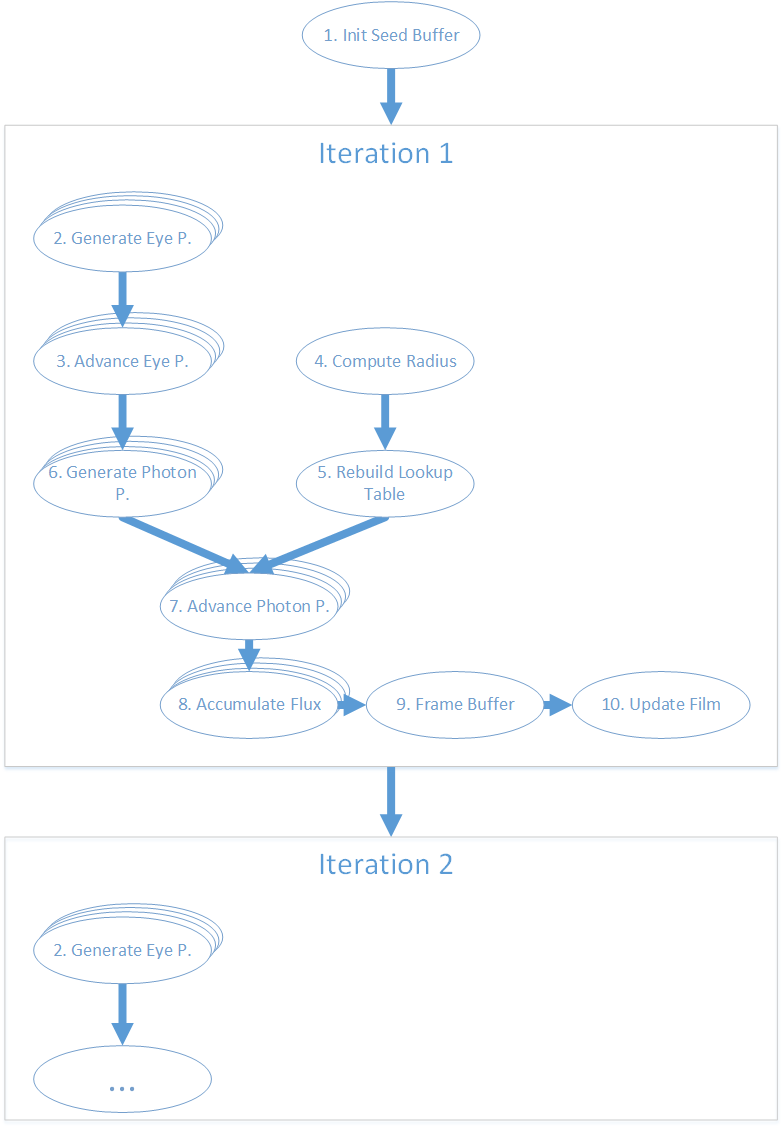
\includegraphics[width=\textwidth]{visio/diagram_cpu}
  \caption[Diagram of SPPMPA computational tasks and execution order]{Diagram of the SPPMPA computational tasks and execution order. Tasks \textbf{2}, \textbf{3}, \textbf{6}, \textbf{7}, \textbf{8} can be parallelized. All other are sequential. The SPPMPA algorithm actually allows independent iterations, which is not represented in this diagram.}
  \label{fig:diagram_cpu}
\end{figure}

The remaining tasks are not specified by the photon mapping techniques, but are required for computational purposes. Task \textbf{5} represents an important step to make sure that access to each hit point is done efficiently when tracing the photons. By using a lookup table to index hit points, the average complexity in accessing a single hit point is lowered to $O(1)$.

\end{document}
